\chapter{導入} \label{cha:introduction}

\section{光生成反応}

宇宙線ミューオンが核子(陽子, 中性子)と起こす反応に光生成反応がある.
この反応は核子とミューオンから出てくる光子との反応である.
また, この反応によりできるハドロン中間状態($\gamma ^* N$)は, 核子(N)と光子($\gamma$)の不変質量が小さい場合は短寿命の共鳴状態に近い.
また, 終状態にはハドロンの中でも最も質量の小さいパイオン($\pi$)と核子(p,n)の2つの粒子が出てくると期待される.
本実験では荷電粒子が2つ出てくる$\pi,p$が生成される反応に着目する.

\begin{figure}[H]
	\centering
	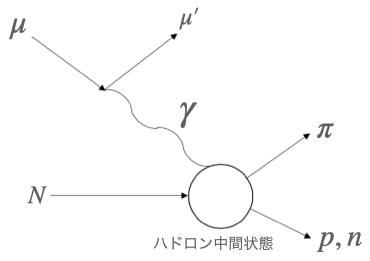
\includegraphics[width=10cm]{img/diagram_photoproduction.png}
	\caption{光生成反応のダイアグラム}
\end{figure}